\chapter{Experimental Results\label{chap:exp-results}}

In this chapter, we will summarize the results of various experiments
conducted with all the solutions presented in Chapter~\ref{chap:data_struct_dev}.
First we will compare the results of some experiments made both in PRACTISE 
and in the Linux kernel. Those experiments show the ability of PRACTISE to predict 
the relative performance of different algorithms.
 
Then, we will focus on the scalability of the algorithms presented in
Chapter~\ref{chap:data_struct_dev}: as the number
of the underlying CPUs increases, we will see that the tasks migration mechanism
still shows good performance for both \emph{push} and \emph{pull} operations.

Before implementing the algorithms in kernel space, extensive tests
with PRACTISE were conducted. We used the tool to correct all the bugs found by the
checking subsystem (discussed in Section~\ref{sec:PRACTISE_data_struct}). 
Then, we conducted a performance analysis to
understand which solution performs best in the user space simulation. As we
will show in this chapter, each algorithm provides interesting results that
allowed us to reach, step by step, a solution that scales well in every
situation. So, it has been decided to port all the algorithms in kernel space, 
to run a performance test with each of them. Those tests have confirmed once 
again the ability of PRACTISE to predict the relative performance of the code
tested with it.

While porting the algorithms in kernel space, the code developed with PRACTISE 
has undergone very little changes, almost all related to the differences presented
in Table~\ref{tab:lock_compare} in Section~\ref{sec:PRACTISE_event_gen}.
In addition to those, a single modification has to be highlited: in kernel
space we do not have the \texttt{rand} function of the \emph{C standard library},
so the \texttt{kernel\_current\_time} function has been used to obtain a 
pseudo-random value to generate skip list items. For our purpose this function
is sufficient, because we do not need a strong random generator.

\section{Experiments with PRACTISE\label{sec:PRACTISE_exp_setup}}

The aim of the experimental evaluation is to compare performance measures obtained with
PRACTISE with what can be extracted from the execution on a real machine.

Of course, we cannot expect the measures obtained with PRACTISE to compare directly with the
measure obtained within the kernel; there are too many differences between the two execution
environments to make the comparison possible. For example, we can consider the completely different
synchronization mechanisms or the unpredictability of hardware interrupts that the kernel
has to manage. However, comparing the performance of two alternative algorithms
within PRACTISE can give us an idea of their relative performance within the kernel.

In Linux we run experiments on a Dell PowerEdge R815 server equipped with 64GB of RAM, and
4 AMD$^{R}$ Opteron$^{TM}$ 6168 12-core processors running at 1.9 GHz, for a total of 48 cores.
We generated 20 random task sets (using the \texttt{randfixedsum}~\cite{Emberson10-WATERS} algorithm) with
periods log-uniform distributed in [10ms, 100ms], per CPU utilisation of 0.6, 0.7 and 0.8
and considering 2, 4, 8, 16, 24, 32, 40 and 48 processors. Then, we ran each task set for 10
seconds using a synthetic benchmark \footnote{rt-app:~\url{https://github.com/gbagnoli/rt-app}}
that lets each task execute for its WCET every period. We varied the number of active CPUs
using the Linux CPU hot plug feature and we collected scheduler statistics through 
the \texttt{sched\_debug} proc file.

The results for the Linux kernel are reported in Figures \ref{fig:kernel-set} and
\ref{fig:kernel-find}, for modifying and querying the data structures, respectively.

\begin{figure}[htbp]
	\centering
	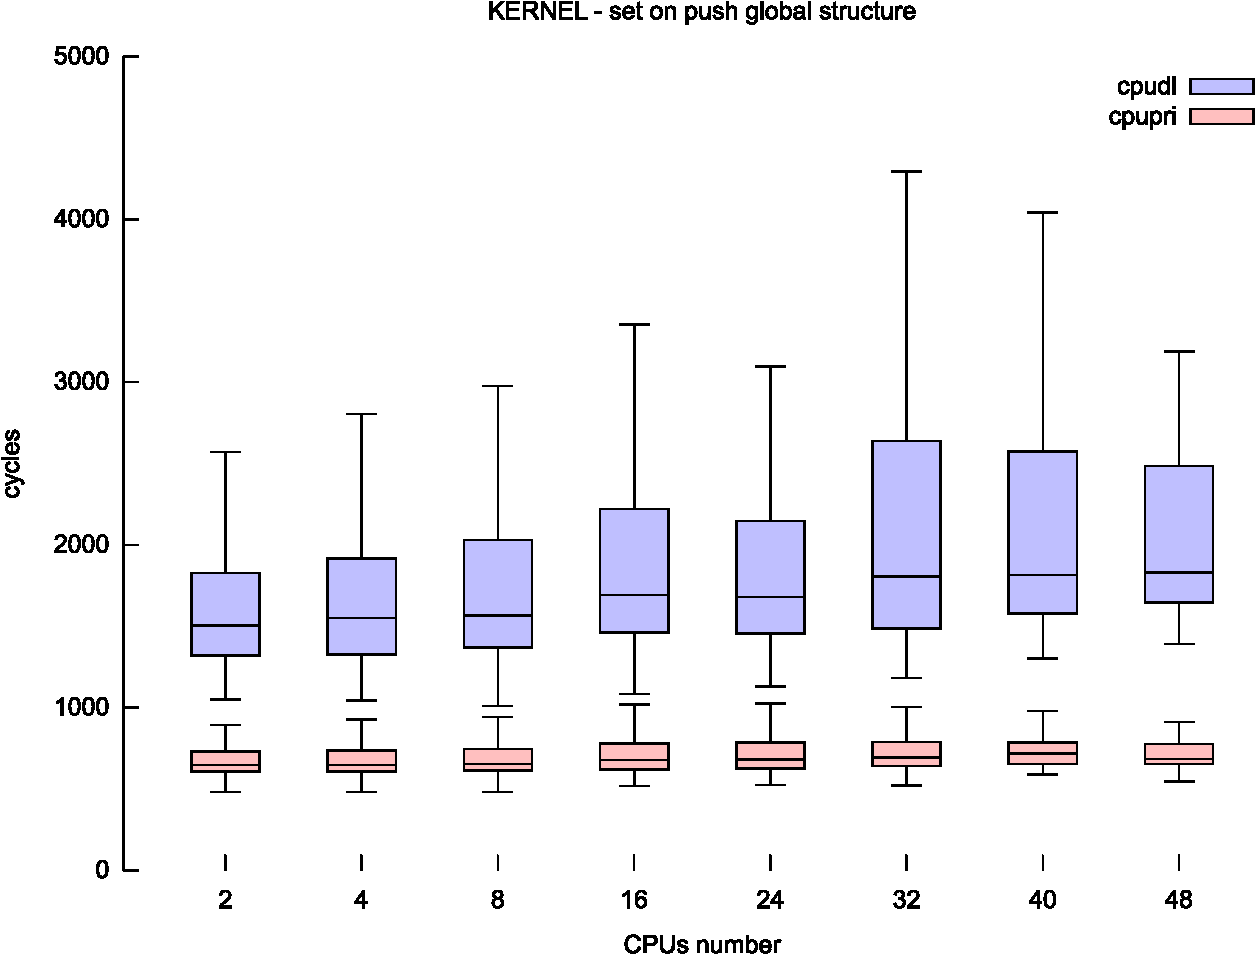
\includegraphics[height=3.5in, keepaspectratio]{images/kernel_set.pdf}
	\caption{Global data structure modify}
	\label{fig:kernel-set}
\end{figure}

\begin{figure}[htbp]
	\centering
	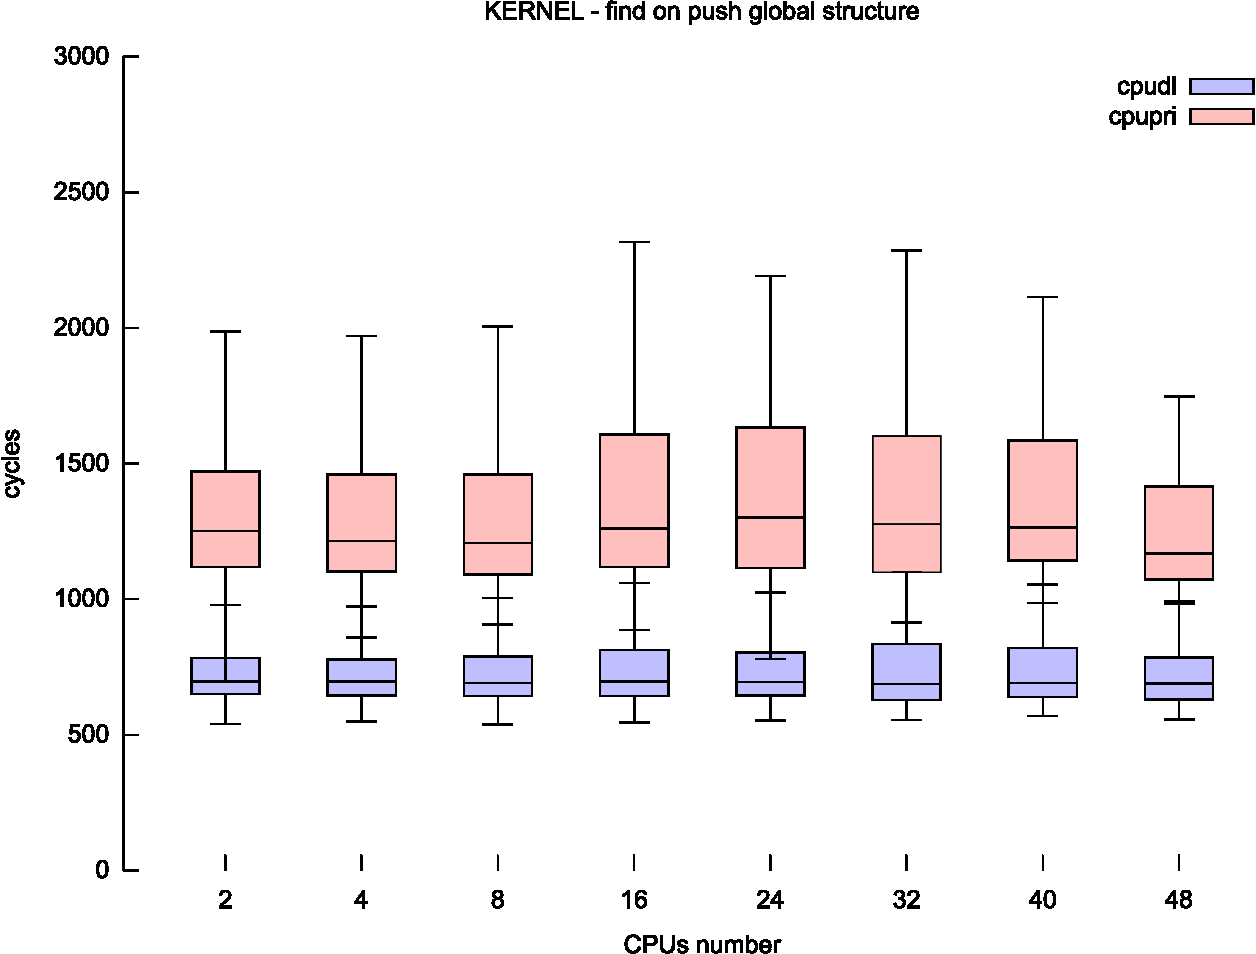
\includegraphics[height=3.5in, keepaspectratio]{images/kernel_find.pdf}
	\caption{Global data structure query}
	\label{fig:kernel-find}
\end{figure}

The figures show the number of cycles (y axis) measured for different number of processors
ranging from 2 to 48 (x axis). The measures are shown in boxplot format: a box indicates all
data comprised between the 25\% and the 75\% percentiles, whereas an horizontal lines 
indicates the median value; also, the vertical lines extend from the minimum to the maximum
value.

In PRACTISE we run the same experiments. As depicted in Section~\ref{sec:PRACTISE_event_gen}
random scheduling events generation is instead part of PRACTISE. We varied the number of
active processors from 2 to 48 as in the former case.

We set the following parameters: 10 milliseconds of thread cycle; 20\% probability of new
arrival; 10\% probability of finish earlier than deadline (for \emph{cpudl} data structure)
or runtime (for \emph{cpupri} data structure); 70\% probability of doing nothing. These
probability values lead to rates of about 20 task activation / (core * s), and 20 task blocking
/ (core * s).

The results are shown in Figures \ref{fig:practise-set-rm} and \ref{fig:practise-set-edf} 
for modifying the \emph{cpupri} and \emph{cpudl} data structures, respectively; and in 
Figures \ref{fig:practise-find-rm} and \ref{fig:practise-find-edf} for querying the \emph{cpupri} 
and \emph{cpudl} data structures, respectively.

\begin{figure}[htbp]
	\centering
	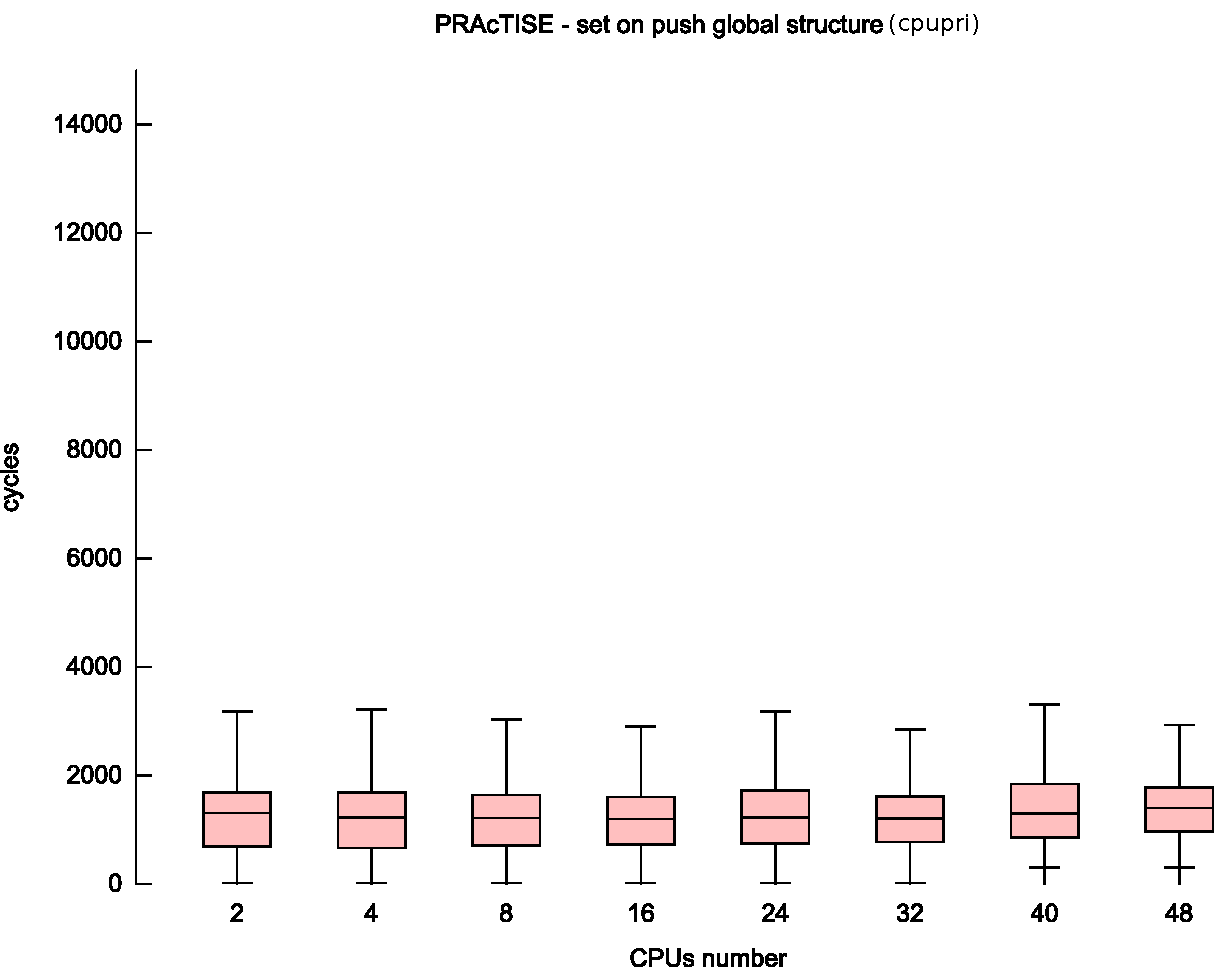
\includegraphics[height=3.5in, keepaspectratio]{images/PRACTISE_set_cpupri.pdf}
	\caption{Global data structure \emph{cpupri} modify}
	\label{fig:practise-set-rm}
\end{figure}

\begin{figure}[htbp]
	\centering
	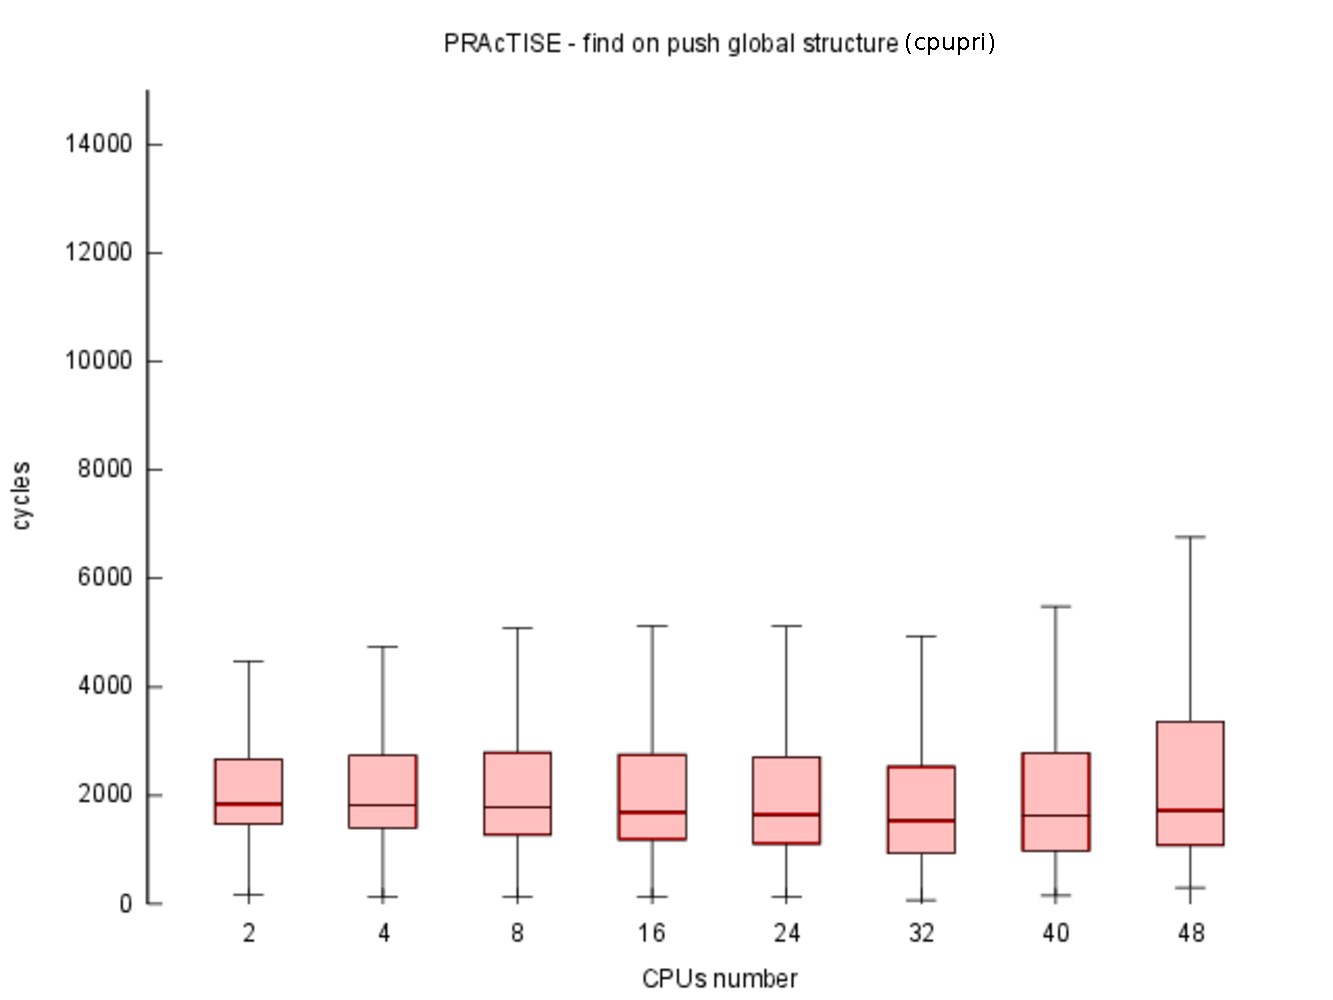
\includegraphics[height=3.5in, keepaspectratio]{images/PRACTISE_find_cpupri.pdf}
	\caption{Global data structure \emph{cpupri} query}
	\label{fig:practise-find-rm}
\end{figure}

\begin{figure}[htbp]
	\centering
	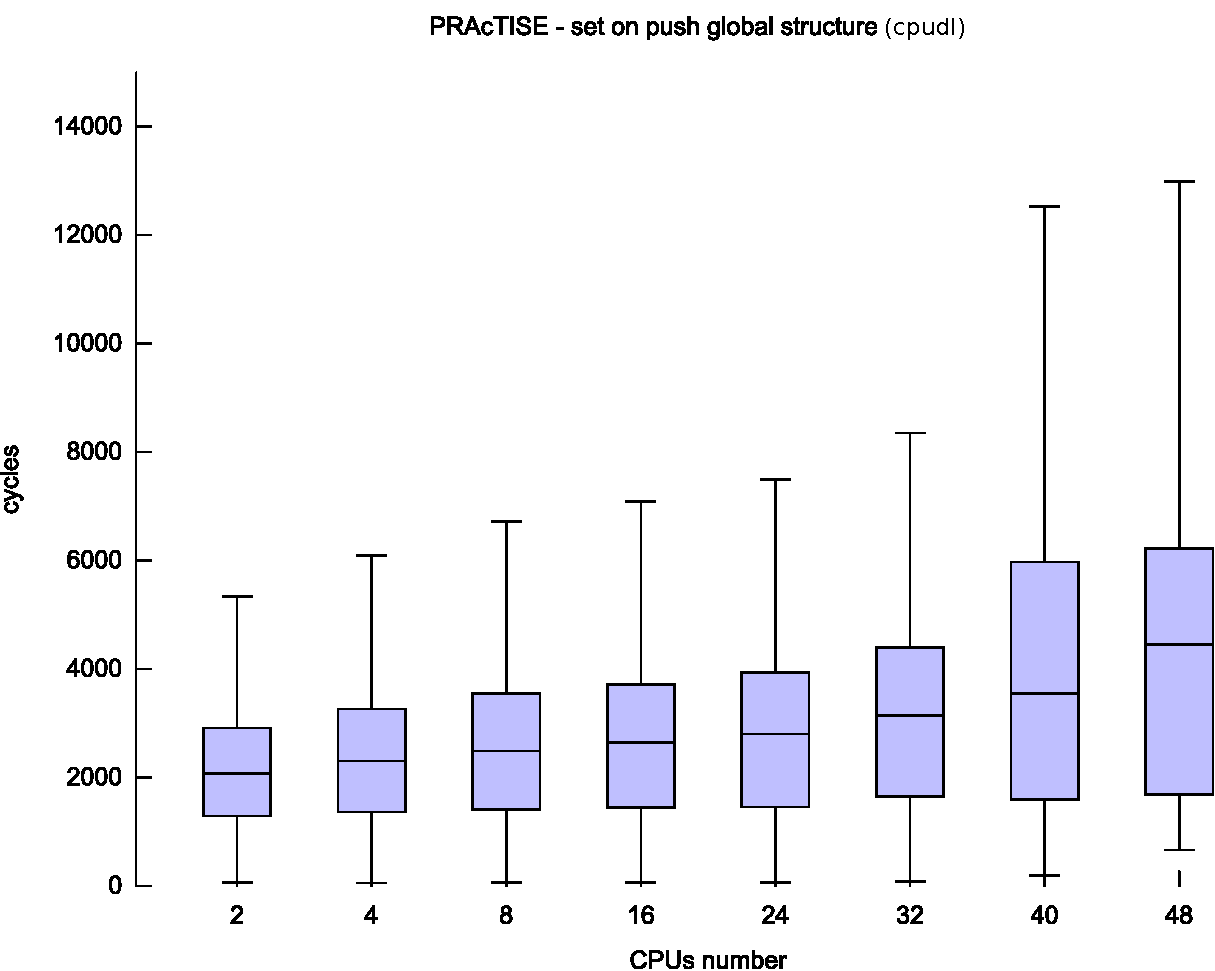
\includegraphics[height=3.5in, keepaspectratio]{images/PRACTISE_set_cpudl.pdf}
	\caption{Global data structure \emph{cpudl} modify}
	\label{fig:practise-set-edf}
\end{figure}

\begin{figure}[htbp]
	\centering
	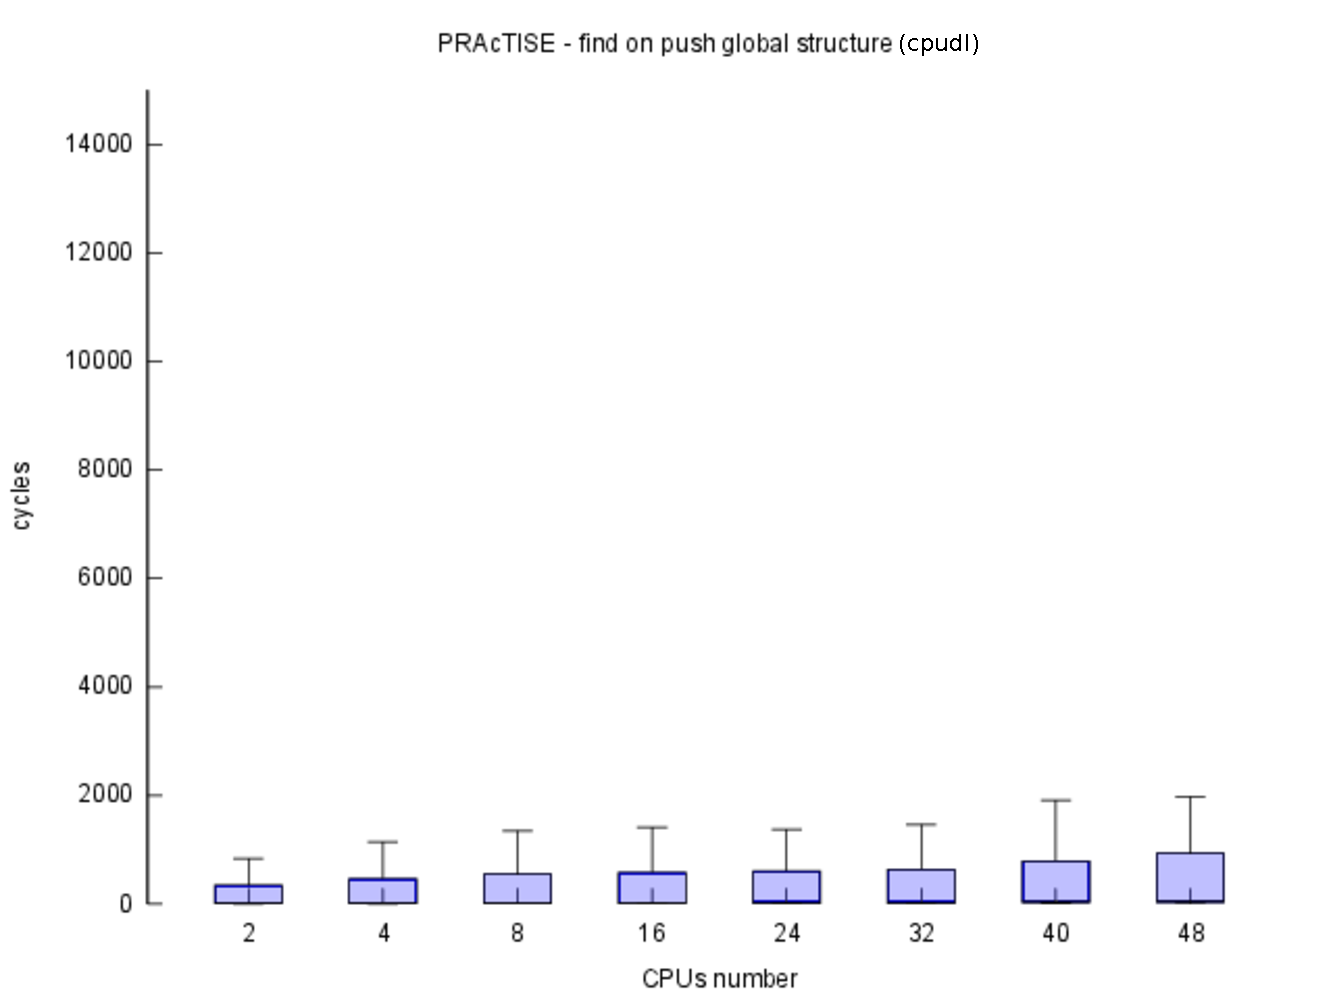
\includegraphics[height=3.5in, keepaspectratio]{images/PRACTISE_find_cpudl.pdf}
	\caption{Global data structure \emph{cpudl} query}
	\label{fig:practise-find-edf}
\end{figure}

Insightful observations can be made comparing performance figures for the same operation
obtained from the kernel and from simulations. Looking at Figure~\ref{fig:kernel-set} we
see that modifying the \emph{cpupri} data structure is generally faster than modifying
\emph{cpudl} data structures: every measure corresponding to the former structure falls
below 1000 cycles while the same operation on \emph{cpudl} takes about 2000 cycles. Same
trend can be noticed in Figures \ref{fig:practise-set-rm} and \ref{fig:practise-set-edf}.
Points dispersion is generally a bit higher than in the previous cases; however median
values for \emph{cpupri} are strictly below 2000 cycles while \emph{cpudl} never goes
under that threshold. We can see that PRACTISE overestimates this measures: in Figure
\ref{fig:practise-set-rm} we see that the estimation for the \emph{set} operation on
\emph{cpupri} are about twice the ones measured in the kernel; however, the same happens
for \emph{cpudl} (in Figure~\ref{fig:practise-set-edf}); therefore, the relative
performance of both does not change.

Regarding query operations the ability of PRACTISE to provide an estimation of actual
trends is even more evident. Figure~\ref{fig:practise-find-edf} shows that a \emph{find} 
on \emph{cpudl} is generally more efficient than the same operation on \emph{cpupri}; this
was expected, because the former simple reads the top element of the heap. Comparing
Figure~\ref{fig:practise-find-rm} with Figure~\ref{fig:practise-find-edf} we can state 
that latter operations are the most efficient also in the simulated environment.
As a concluding use-case, it is worth mentioning that PRACTISE has already been used as a
testing environment for the last SCHED\_DEADLINE release on the LKLM\footnote{LKLM 
(Linux Kernel Mailing List) thread available at: \url{https://lklm.org/lklm/2012/4/6/39}}.
The \emph{cpudl} global data structure underwent major changes that needed to be verified.
The tested code has been finally merged within the patch set.

\section{Kernel Experiments\label{sec:exp_setup}}

Regarding the kernel experiments, since the results for the different values 
of CPU utilization are very similar, in the subsequent sections we are 
going to show only the graphs related to task sets with a U value of 0.8.

We will focus on the graphs related to the performance of the \texttt{cpudl} data
structures, that is: the CPU cycles of the \emph{find} operation and the \emph{set}
operation. We will show the number of \emph{push} and \emph{pull} 
operations and we will point out the benefit of using a \texttt{cpudl} data structure
to speed up the pull operations.

\section{Comparison between max-heap and skip list\label{sec:heap_vs_skiplist}}

In this section we are going to focus on the \emph{push} operation: we will compare
the \texttt{cpudl} max-heap with the skip list one.

The results are shown in Figure~\ref{fig:heap_skiplist_find}. 

We can see that the \emph{find} operation is always faster in the skip list
implementation: the median value is always under 600 CPU cycles, while the max-
heap never goes under that threshold. Both implementations are not affected by
the increase in the CPUs number: we can see that the results are the same from
2 to 48 CPUs. This shows that they are both scalable.

\begin{figure}[htbp]
    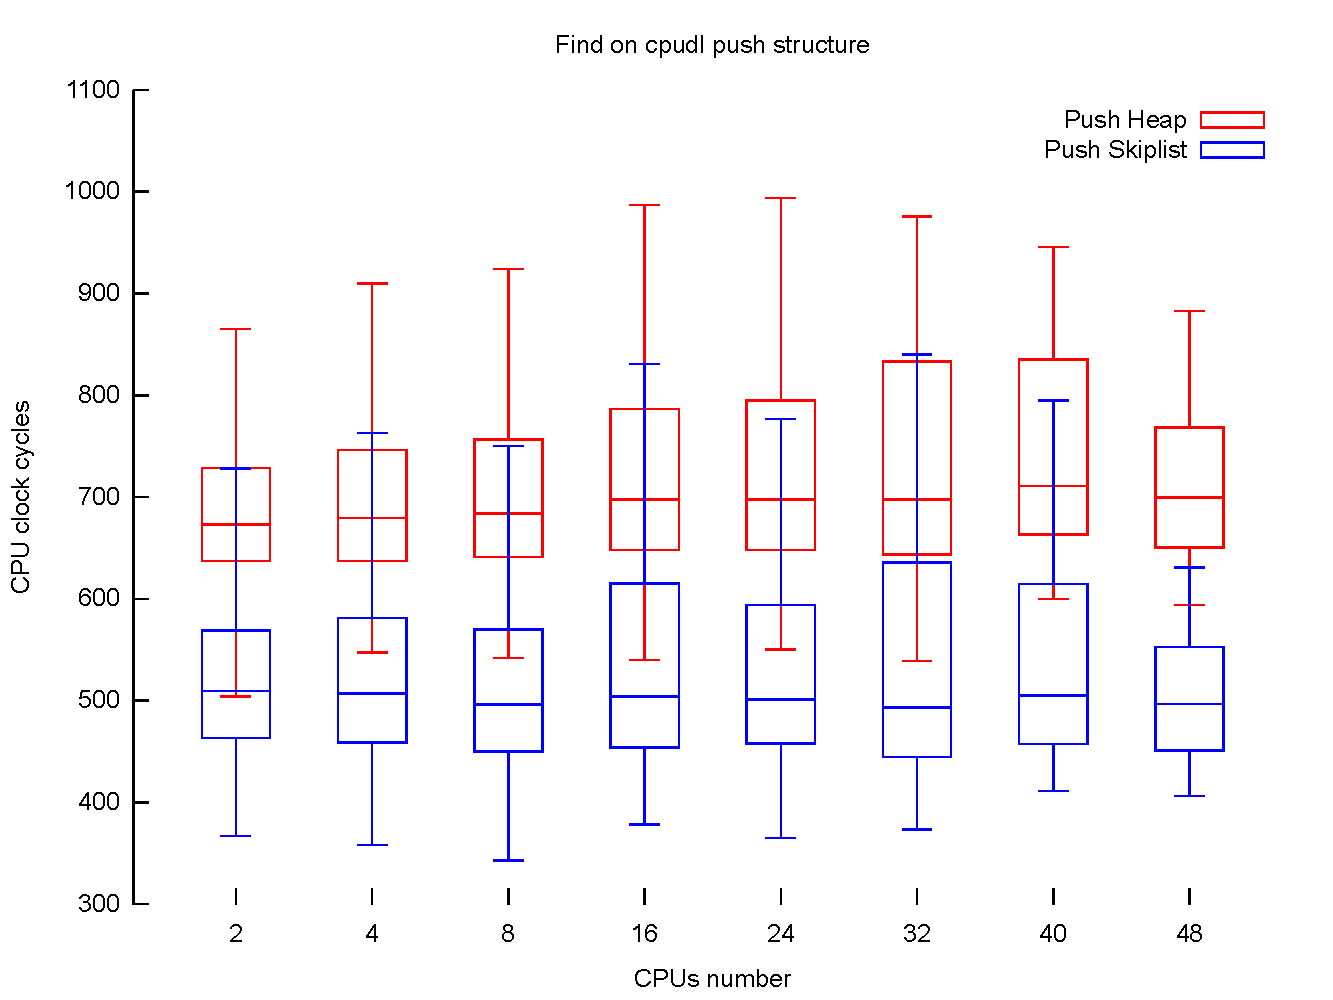
\includegraphics[width=\columnwidth]{images/heap_skiplist_find.pdf}
    \caption{\emph{set} operation on max-heap and skip list kernel}
    \label{fig:heap_skiplist_find}
\end{figure}

Regarding the \emph{set} operation, the result is reversed 
(Figure~\ref{fig:heap_skiplist_set}): we
see that the max-heap is very fast and never exceeds the 2000 cycles threshold.
We can see that also the scalability of this solution is good: as the number of
CPUs increases, the heap still performs quite well, even if a slight worsening
can be noted when the CPUs are 24 or more.

\begin{figure}[htbp]
    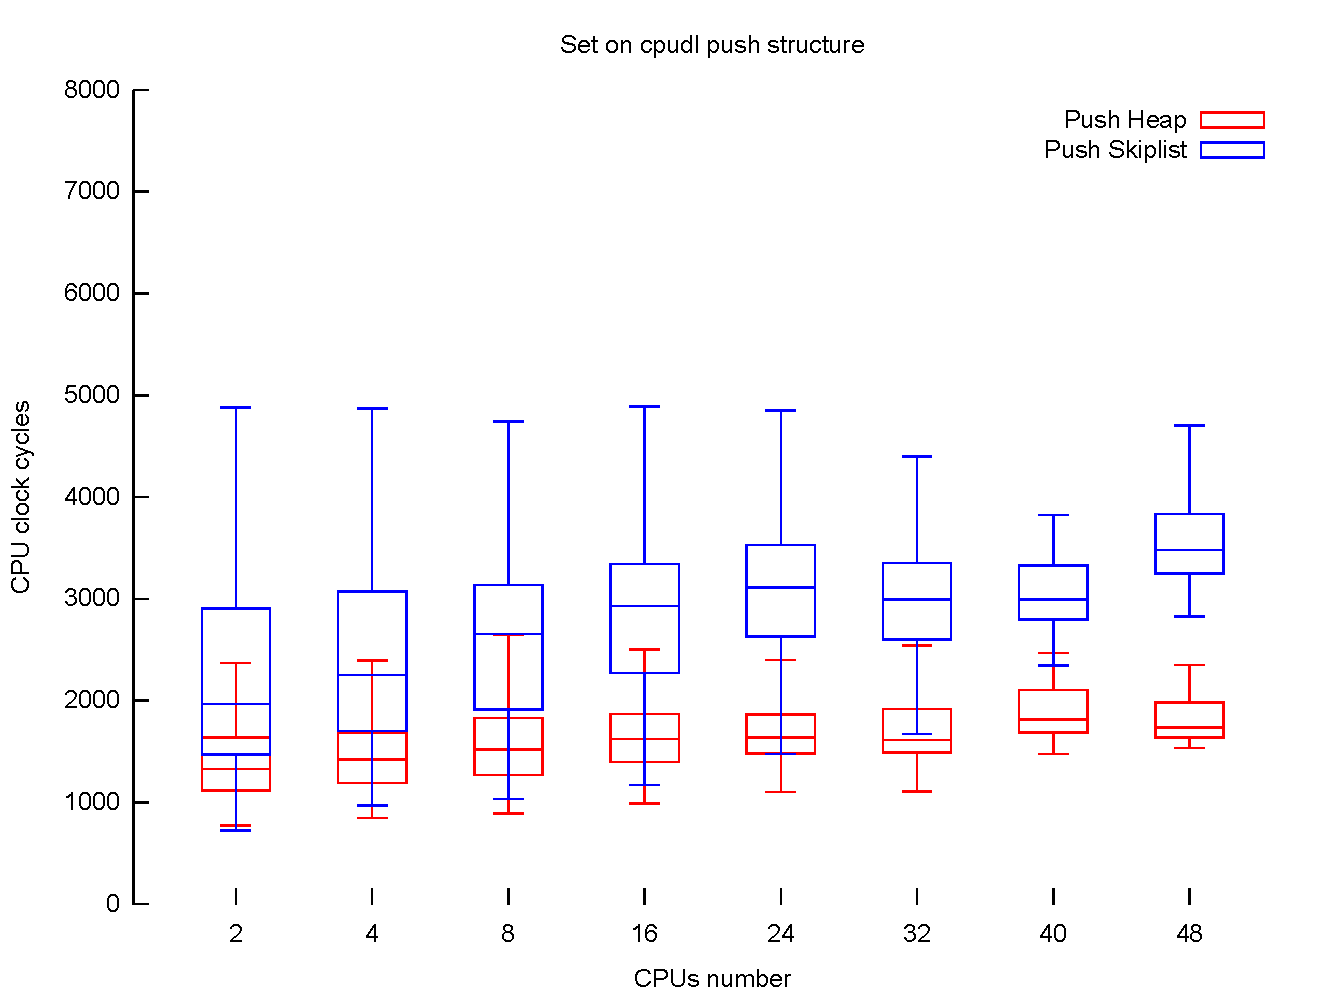
\includegraphics[width=\columnwidth]{images/heap_skiplist_set.pdf}
    \caption{\emph{find} operation on max-heap and skip list kernel}
    \label{fig:heap_skiplist_set}
\end{figure}

The skip list implementation is not as fast as the heap in updating the
structure: the number of CPU cycles needed to perform the same operations are
about double. Regarding the scalability, we can see that the operation tends
to slightly slow while the CPUs are more than 16, but still mantains
a good performance even with 48 CPUs.

To perform a fair comparison between the two implementations, we need to know
the number of operations carried out on the data structure. 
In Figure~\ref{fig:heap_skiplist_nr_set} 
and Figure~\ref{fig:heap_skiplist_nr_find} we can see the number of \emph{set} 
and \emph{find} per CPU operations, respectively. Since the number of \emph{set} 
operations greatly exceeds the \emph{find}
one, and since the spread between max-heap and skip list performance is much
wider in the \emph{set} case than the \emph{find} one, we can definitely
state that the heap is a better solution for the \emph{push} operation.

\begin{figure}[htbp]
    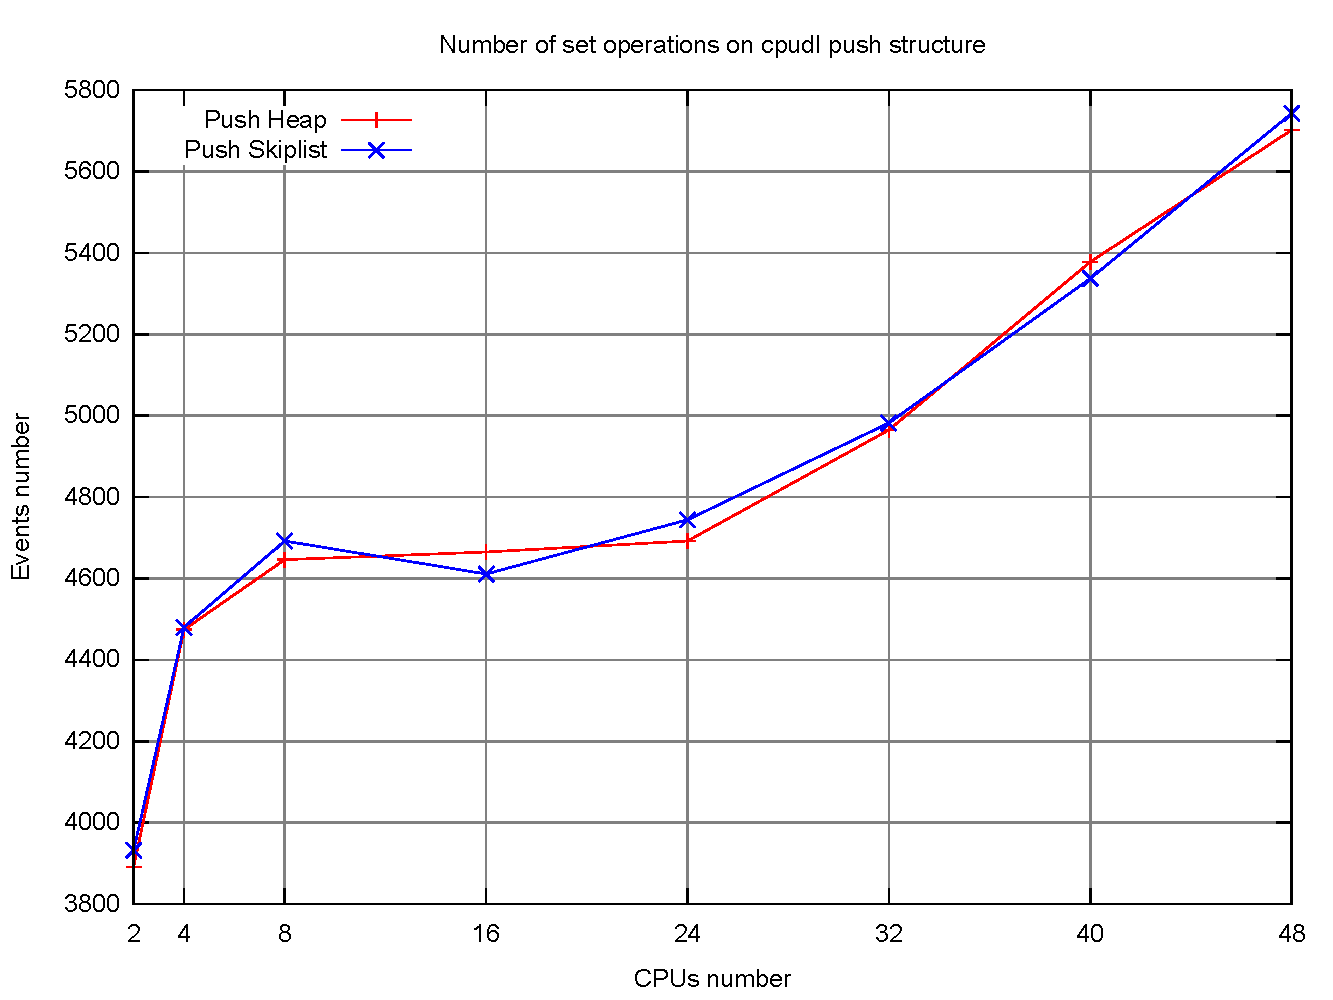
\includegraphics[width=\columnwidth]{images/heap_skiplist_nr_push_set}
    \caption{\emph{set} operations number}
    \label{fig:heap_skiplist_nr_set}
\end{figure}

\begin{figure}[htbp]
    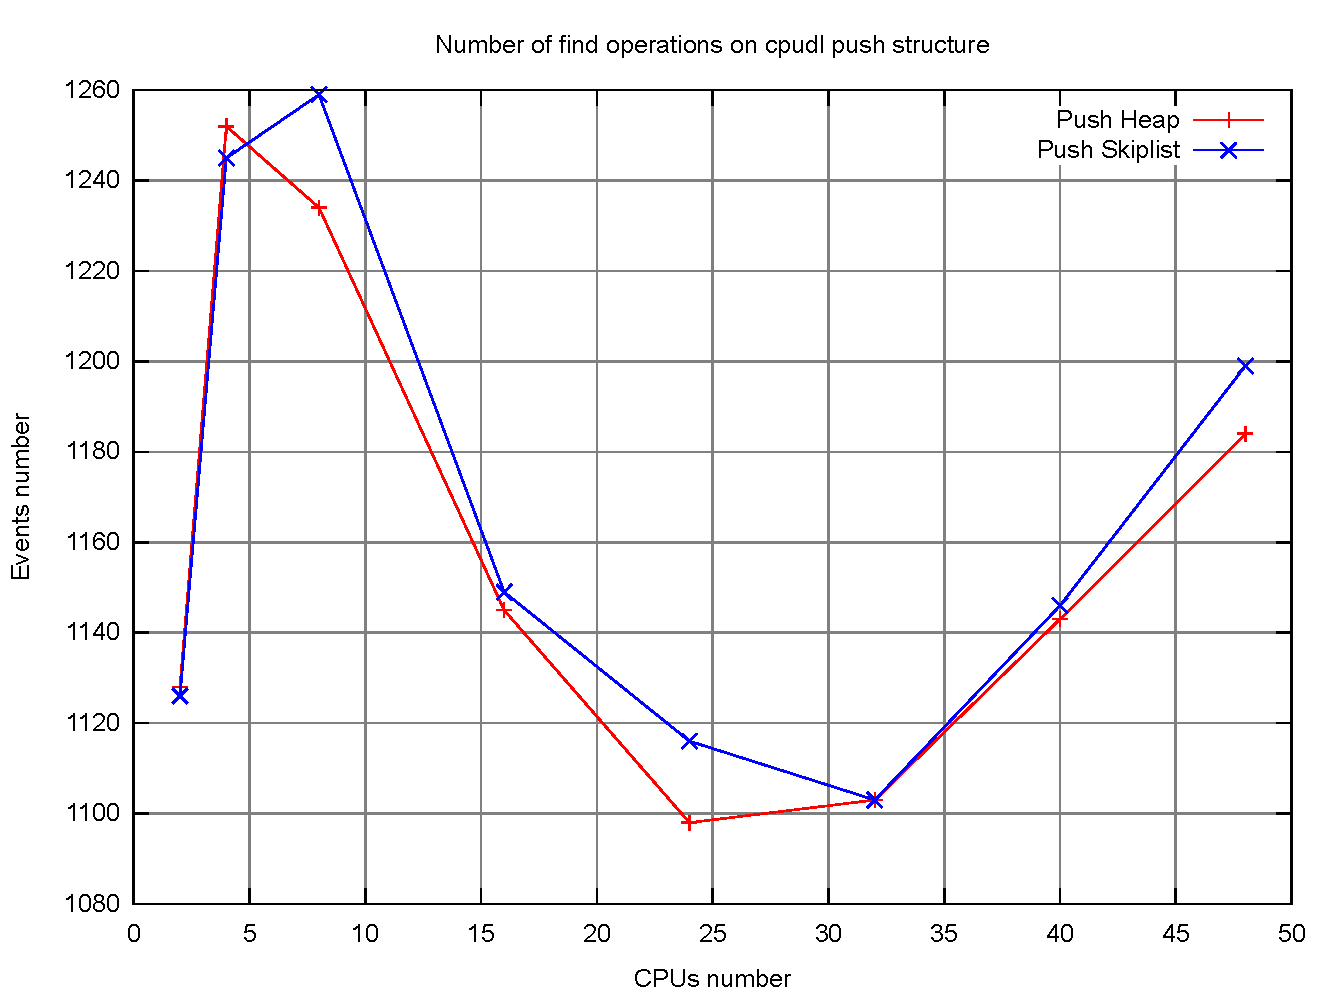
\includegraphics[width=\columnwidth]{images/heap_skiplist_nr_push_find}
    \caption{\emph{find} operations number}
    \label{fig:heap_skiplist_nr_find}
\end{figure}

\section{Improved Pull algorithm performance\label{sec:improved_pull_perf}}

As we have seen in Section~\ref{sec:pull_dl_impl} and in Section~\ref{sec:pull_algo}, 
the current implementation of \texttt{SCHED\_DEADLINE} lacks a data structure 
to speed up the pull operation. So, we decided to address this problem following 
the same approach developed for the push operation. We chose the skip list 
implementation of the \texttt{cpudl} data structure and, with a kernel modified
as such, we conduct the same experiments described in Section~\ref{sec:PRACTISE_exp_setup}.\\
The results are shown in Figure~\ref{fig:cpudl_pull_nr_pushed_away} and in 
Figure~\ref{fig:cpudl_pull_nr_pulled_here} where we can see
the number of succesfull per-CPU task migrations due to push and pull operations,
respectively. Regarding the push-related migrations, we see that there is
no difference; on the other hand, since we used a \texttt{cpudl}
data structure also for \emph{pull} operation, there is no need to 
explore all runqueues in the system: so, the number of migrations is lower
for every number of online CPUs.

\begin{figure}[htbp]
    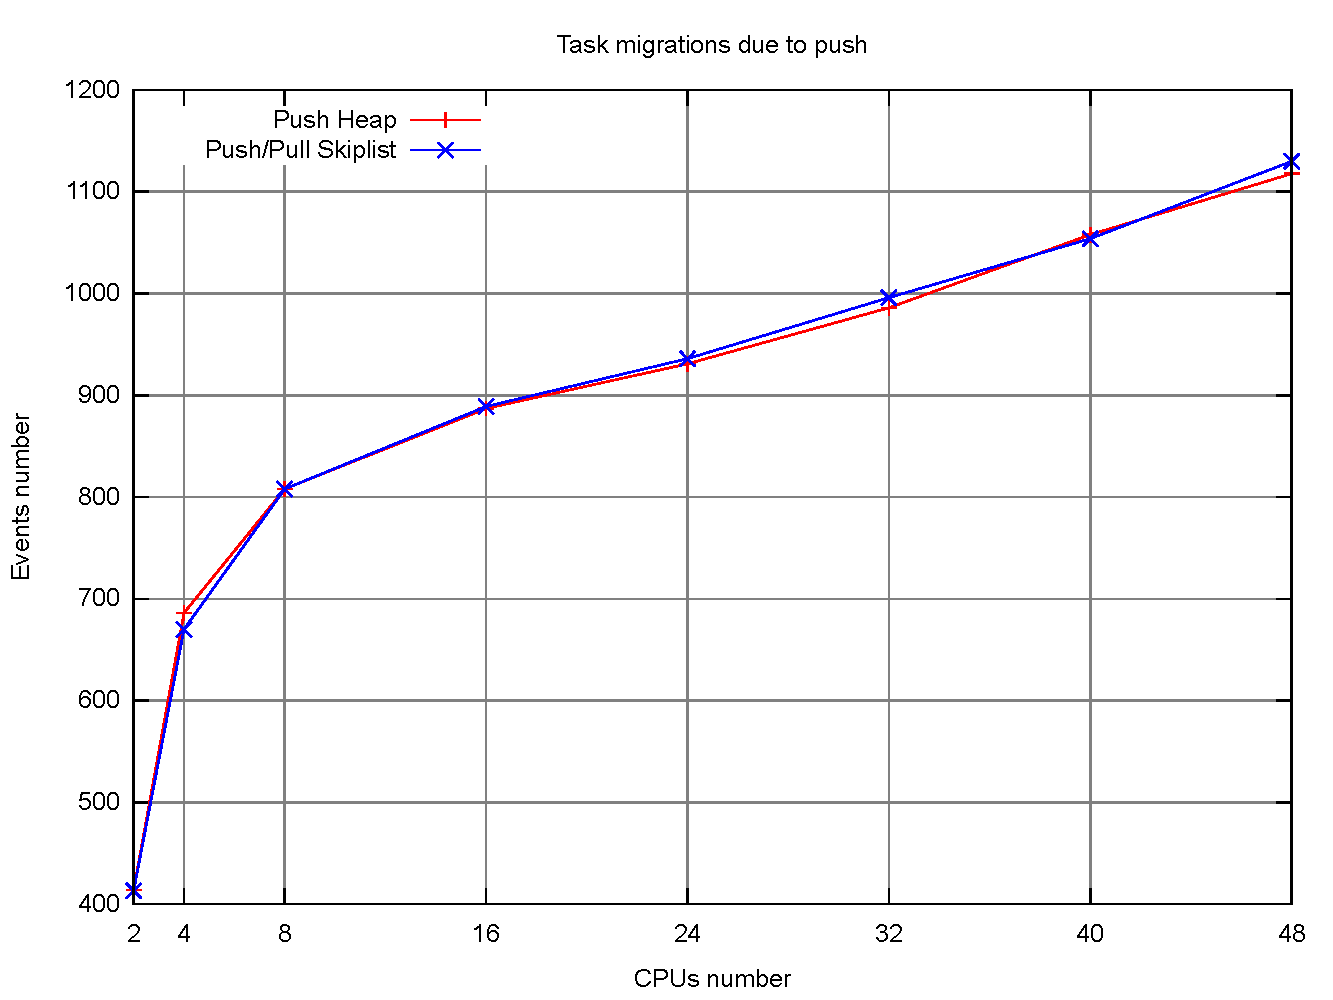
\includegraphics[width=\columnwidth]{images/cpudl_pull_nr_pushed_away}
    \caption{Number of task migrations due to push operation}
    \label{fig:cpudl_pull_nr_pushed_away}
\end{figure}

\begin{figure}[htbp]
    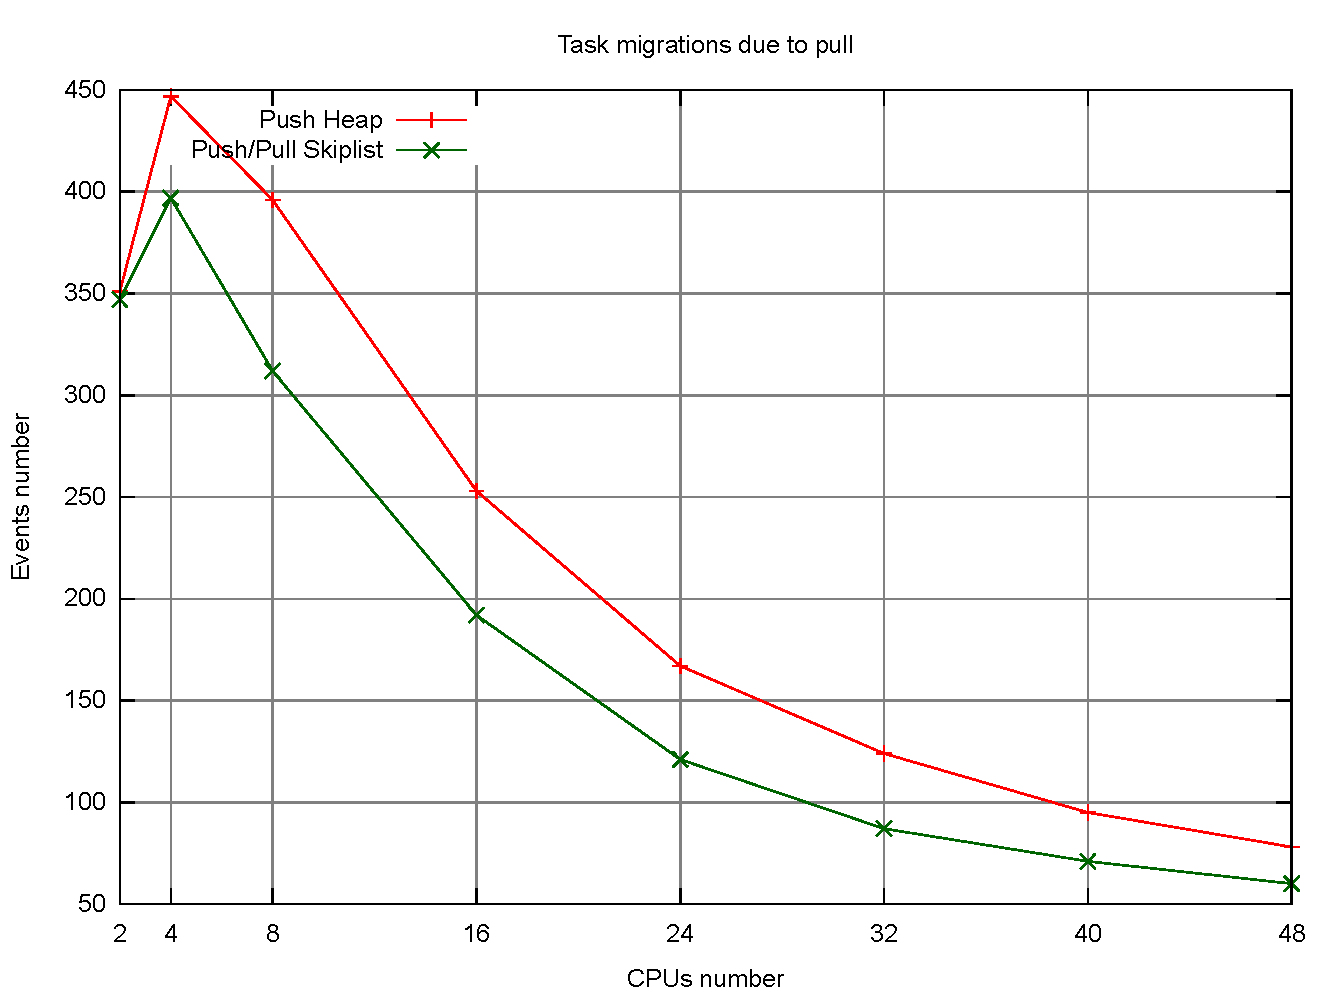
\includegraphics[width=\columnwidth]{images/cpudl_pull_nr_pulled_here}
    \caption{Number of task migrations due to pull operation}
    \label{fig:cpudl_pull_nr_pulled_here}
\end{figure}

\section{Bitmap flat combining performance\label{sec:bm_fc_perf}}

In this section we discuss the performance of
the bitmap flat combining solutions. This implementation is the basis
for the fastcache algorithm.

In Figures~\ref{fig:bm_fc_push} and \ref{fig:bm_fc_pull} we can observe 
the performance related to the push and the pull operations, respectively.
Each graphs contains two figures: the \emph{find} operation 
results on the top half and the \emph{set} operation results
on the bottom half.

\begin{figure}[htbp]
    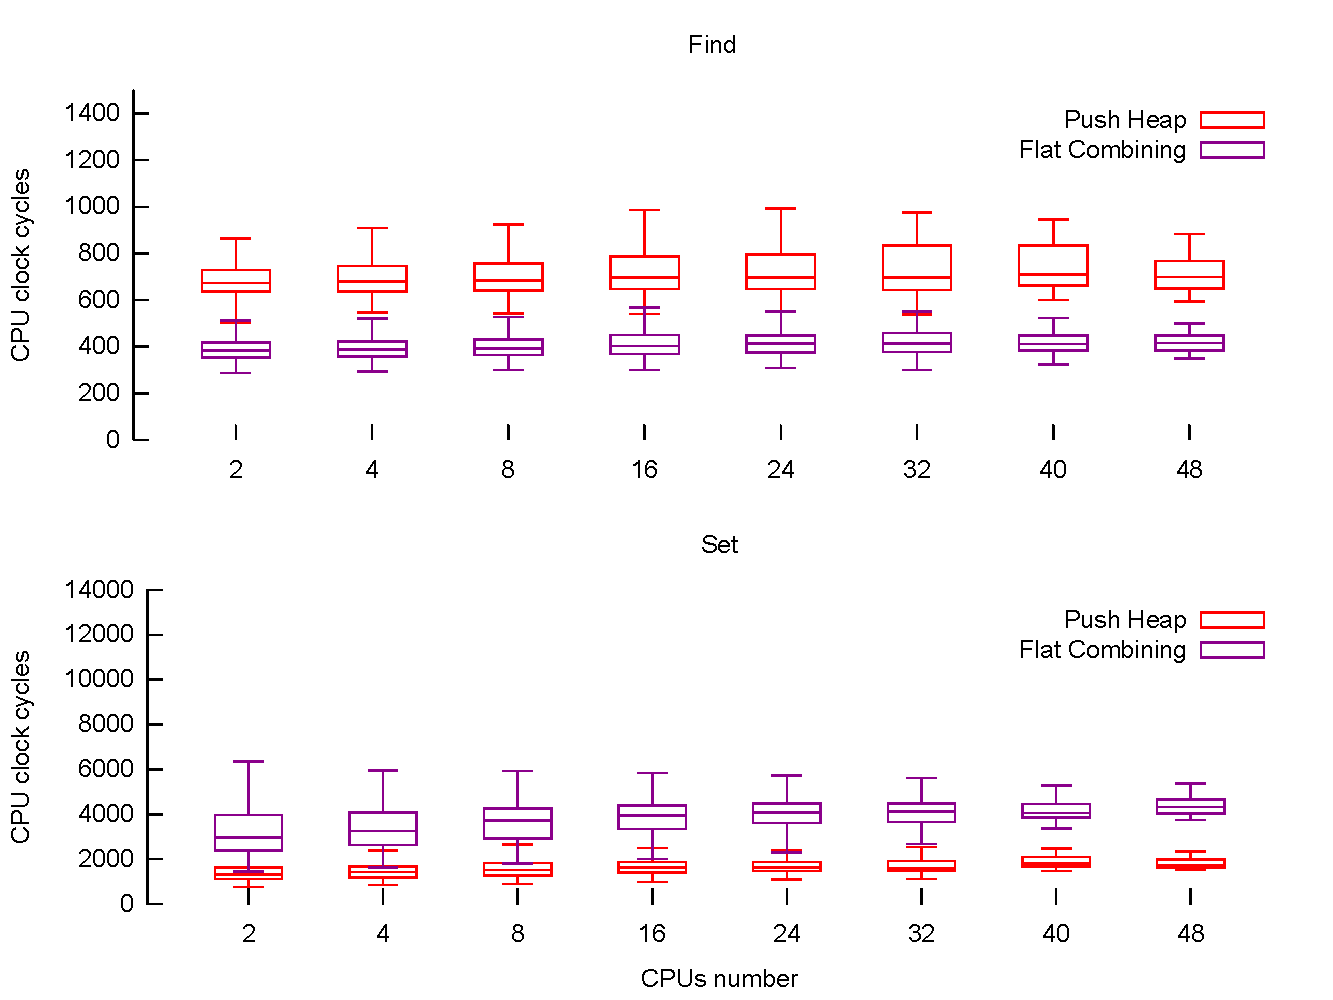
\includegraphics[width=\columnwidth]{images/bm_fc_push}
    \caption{Bitmap flat combining push performance}
    \label{fig:bm_fc_push}
\end{figure}

\begin{figure}[htbp]
    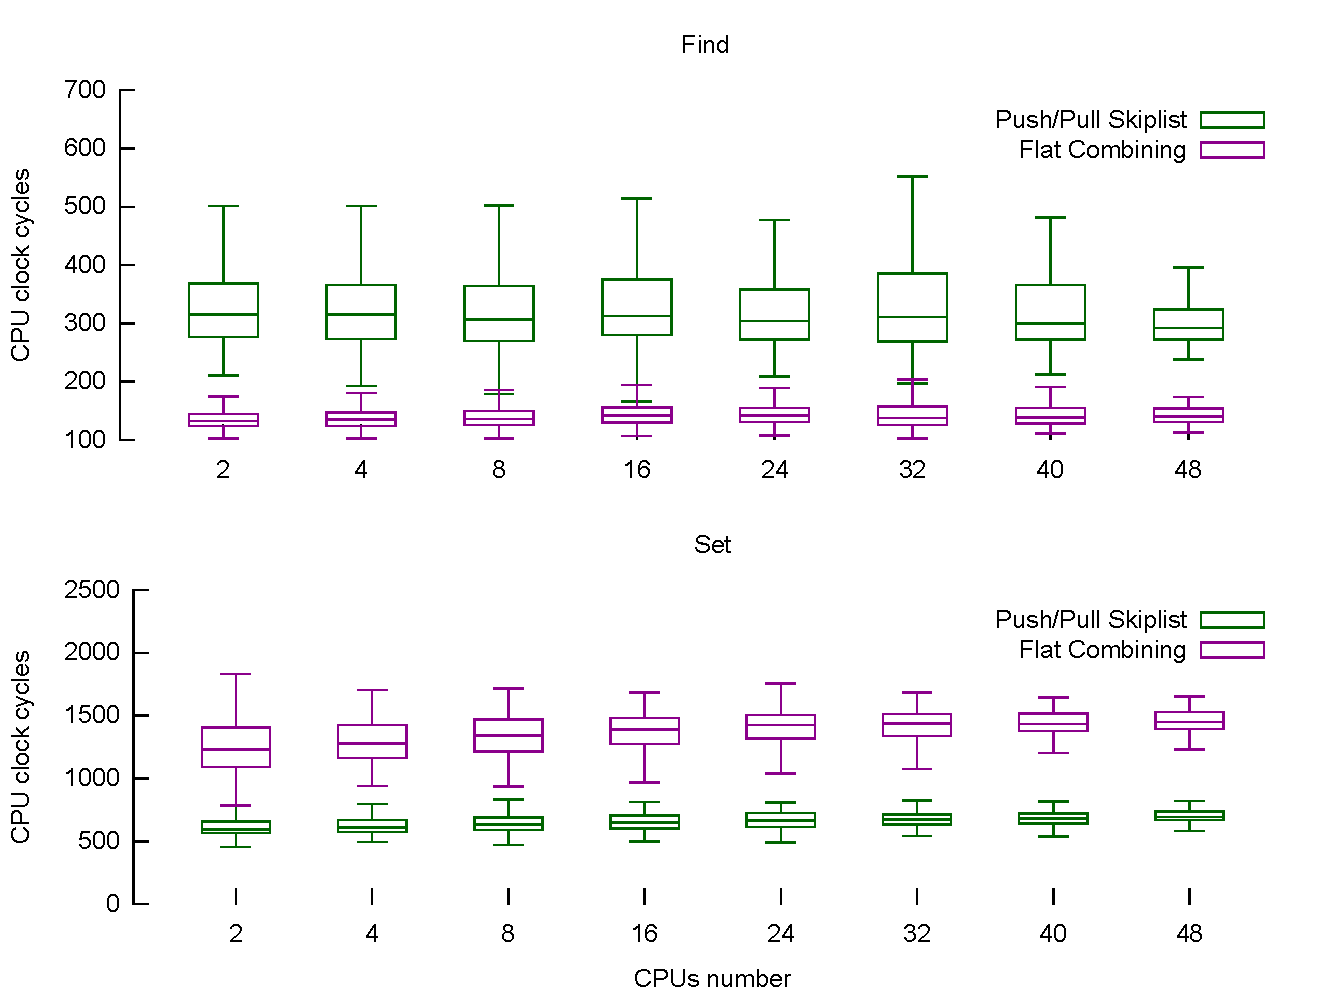
\includegraphics[width=\columnwidth]{images/bm_fc_pull}
    \caption{Bitmap flat combining pull performance}
    \label{fig:bm_fc_pull}
\end{figure}

Regarding the push operation, we compared the bitmap flat combining
with the best current solution: the max-heap. We can see that,
as with the skip list, flat combining reaches very high performance in
the \emph{find} operation. This is due to the best CPU cached value:
if the cache is valid, we can immediately return that CPU index, so
the operation is very fast. The \emph{set} operation is instead slower
for the bitmap flat combining solution. More importantly, we can see
that the performance doesn't scale as well as with the max-heap:
with an increasing number of CPUs, the spread between the two solutions
is even more evident. With 48 online CPUs, the bitmap flat combining
overcomes the 4000 CPU cycles threshold, while the max-heap remains
under 2000 CPU cycles.

Regarding the pull operation, the trend is the same for both \emph{find}
and \emph{set} operations. Here we have to point out that the comparison
is done with the skip list as the improved pull algorithm has been tested
with such data structure.

In conclusion, we see how the cache mechanism, initially introduced
to keep the \emph{cpudl} updated among the underlying runqueues status,
makes the solution very fast for the \emph{find} operation, however, the
flat combining framework is not adequate for the \emph{set} operation.
If we consider the results for the single-lock skip list another time,
we can see how flat combining is even worse than that. This means that
the underlying mechanism to defer work on the data structure puts a non
negligible overhead.

\begin{figure}[htbp]
    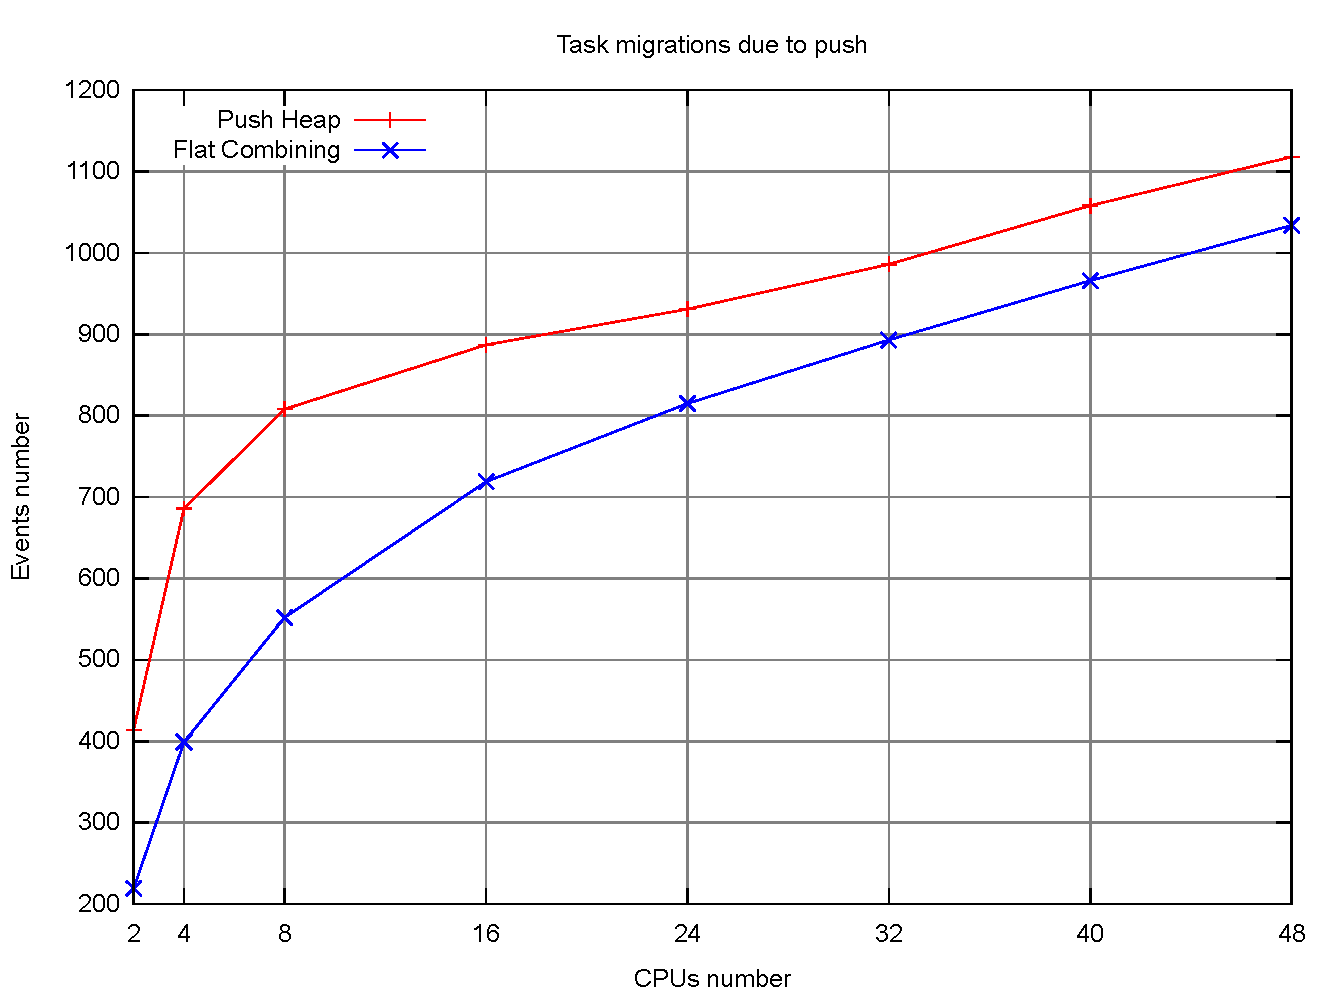
\includegraphics[width=\columnwidth]{images/bm_fc_pushed_away}
    \caption{Number of successfull push operations}
    \label{fig:bm_fc_pushed_away}
\end{figure}

Another insightful observation can be made referring to 
Figure~\ref{fig:bm_fc_pushed_away},
where the number of successfull per CPU push operations is showed. In the
graph the max-heap and the flat combining are compared. As we can see,
the latter has a lower number of succesfull migrations: since we
did not change the push mechanism, then the work
deferring mechanism is the responsible. Hence, the data structure 
cannot correctly represents the runqueues status under certain conditions.
This is a notable drawback that highlights the inadequacy of this
implementation.

\section{Fastcache performance\label{sec:fastcache_perf}}

As discussed in the previous sections, a good solution that aims at
speeding up the task migration mechanism, has to achieve very high performance
in the \emph{set} operation. We have seen how the cache introduced
with flat combining offers good performance in the \emph{find} operation,
but the way this cache is filled after being invalidated overcomes that
benefit. With fastcache	(see Section~\ref{sec:Fastcache}), we try to focus on the cache mechanism,
refilling that with a very light-weight algorithm while ensuring that
the \emph{set} operation related work will be done immediately.

In Figure~\ref{fig:fastcache_push} we can see the performance of
the \emph{find} (top half) and \emph{set} (bottom half) push related
operations.

\begin{figure}[htbp]
    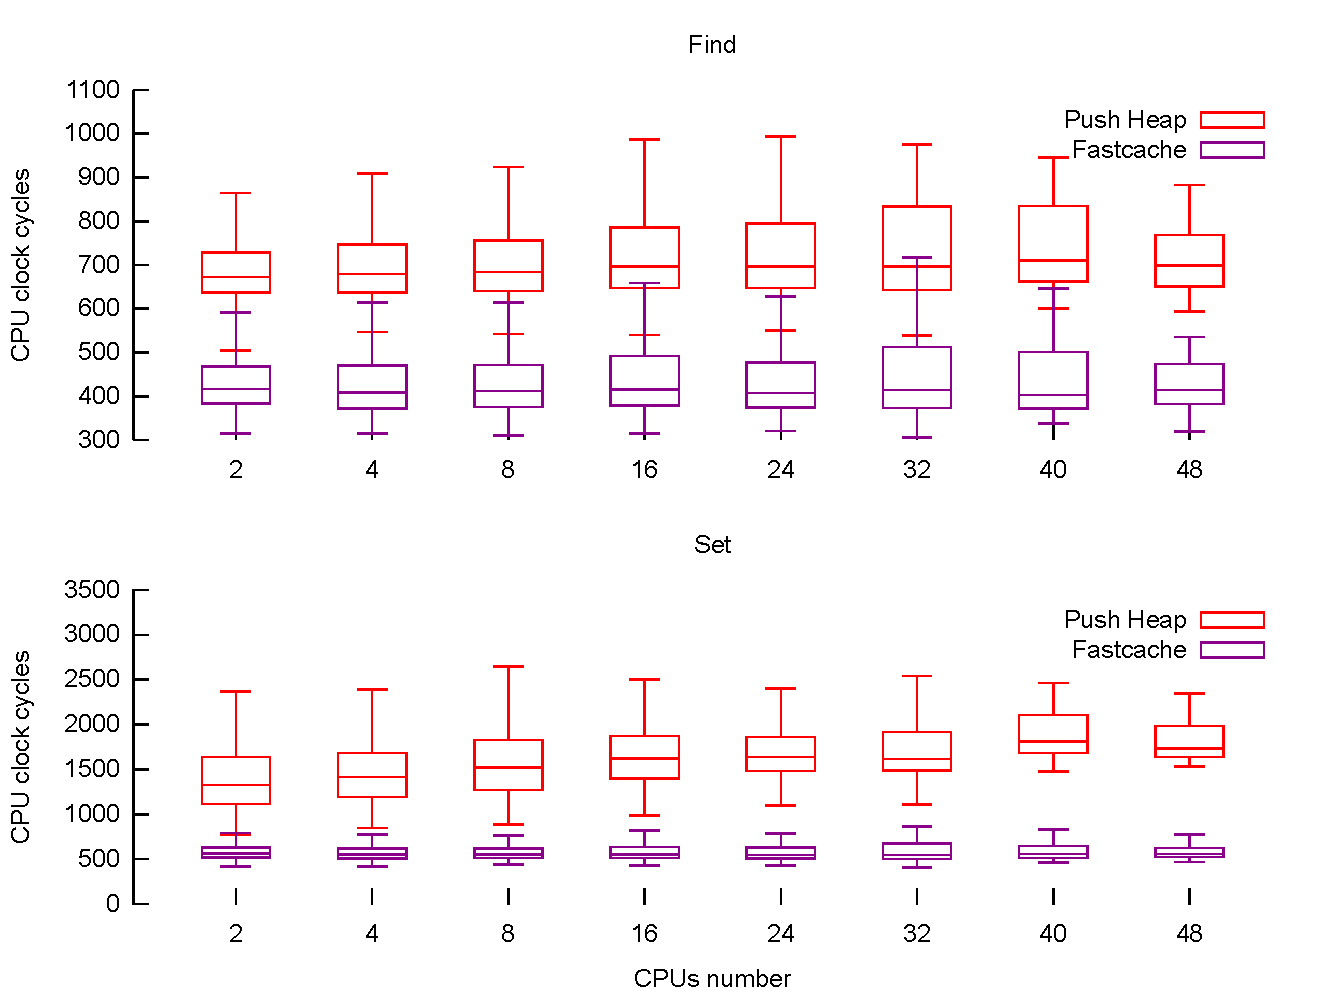
\includegraphics[width=\columnwidth]{images/fastcache_push}
    \caption{Fastcache push performance}
    \label{fig:fastcache_push}
\end{figure}

As usual, we compare fastcache with the max-heap, the fastest solution
for the push operation. As we can see, fastcache overcomes the previous
algorithm, both in the \emph{find} and the \emph{set} operations. The graph related
to the latter operation is the most important: we can see that the trend
remains flat as the number of the CPUs increases. In fact, the spread
between the two graphs is more and more evident increasing the number
of CPUs. Considering the 48 CPUs results, we can see how fastcache
performs the \emph{set} operation in about 600 CPU cycles, while the max-heap
takes more then the 1500 CPU cycles.

The results for the pull operation, showed in Figure~\ref{fig:fastcache_pull},
are quite similar: we see how fastcache, compared to the skip list, 
tends to be always faster.

Also here we can see that the trend of the \emph{set} operation is not 
as flat as the analogous one for push. This phenomenon can be explained 
looking at the number of successfull migration due to push and pull, 
respectively, as shown in Figures~\ref{fig:fastcache_pushed_away} and 
\ref{fig:fastcache_pulled_here}.

\begin{figure}[htbp]
    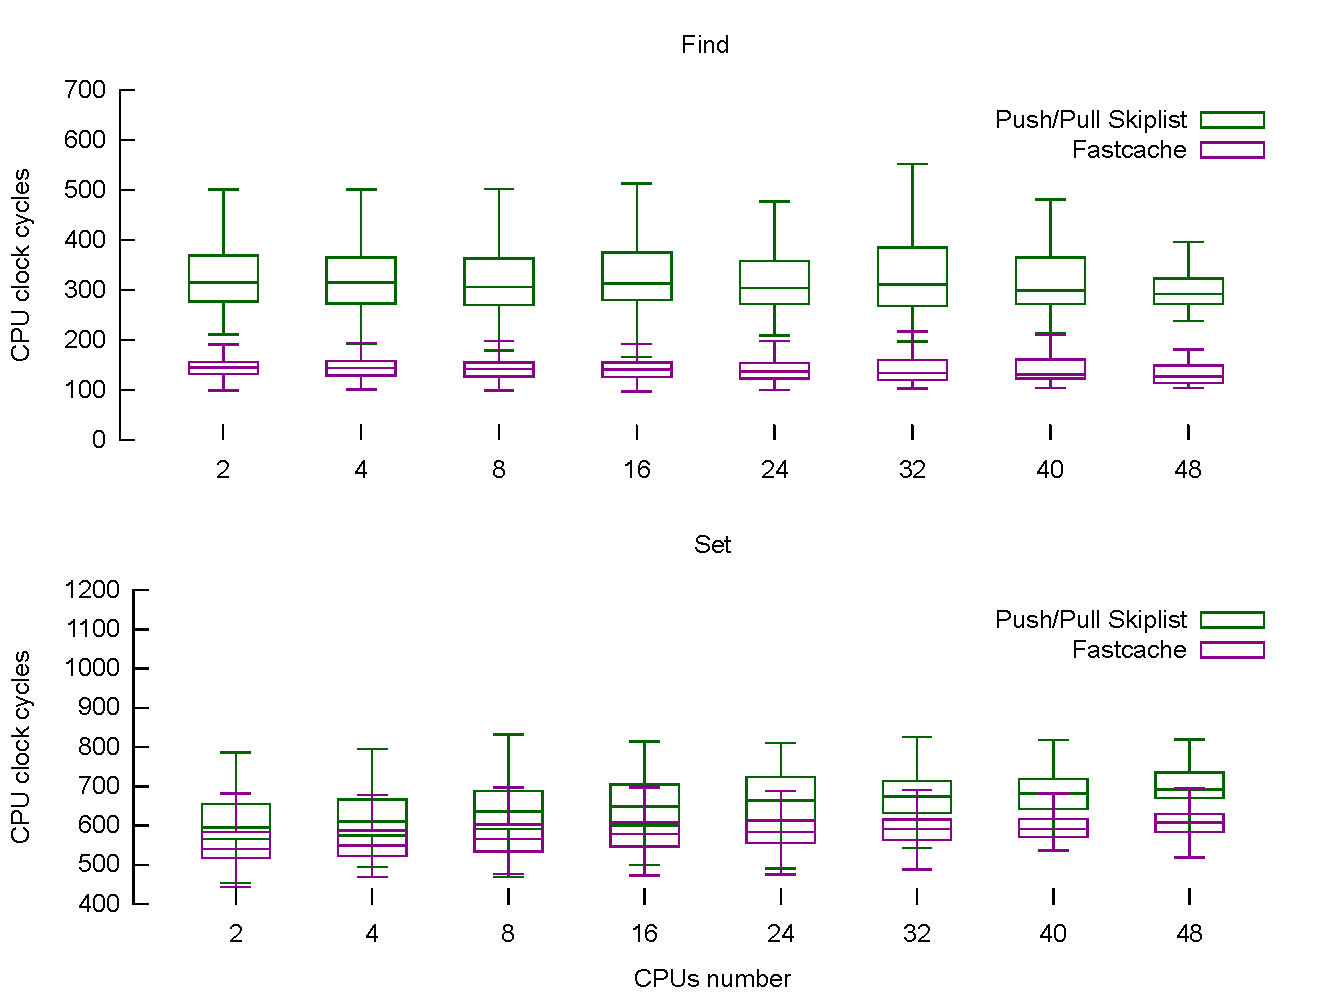
\includegraphics[width=\columnwidth]{images/fastcache_pull}
    \caption{Fastcache pull performance}
    \label{fig:fastcache_pull}
\end{figure}

We can see that the number of task migrations 
due to the push operation, presented in the former figure, greatly overcomes 
the pull related one, in the latter figure.

\begin{figure}[htbp]
    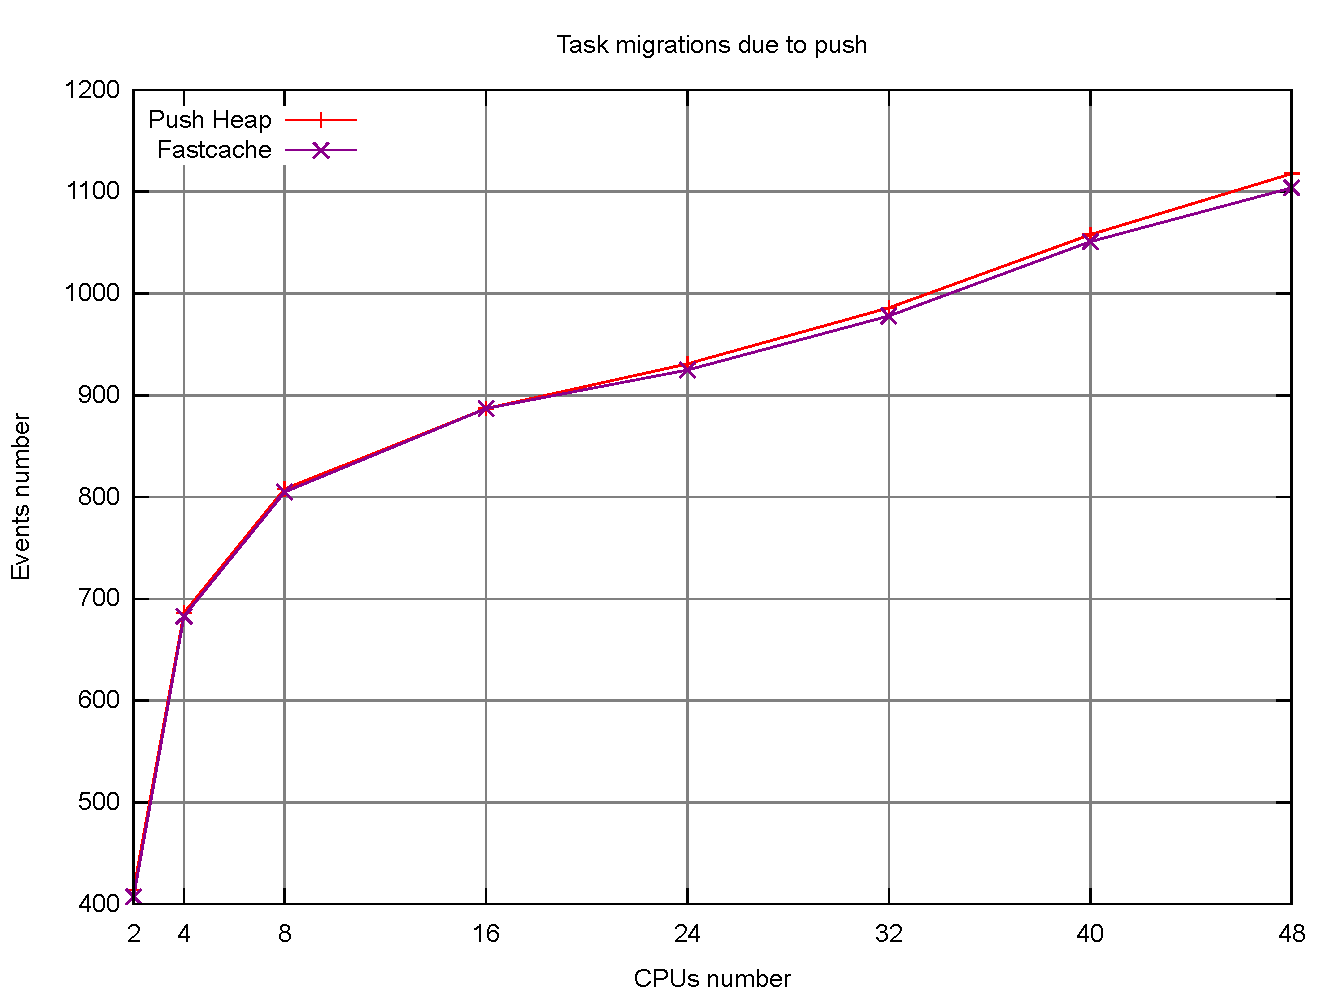
\includegraphics[width=\columnwidth]{images/fastcache_pushed_away}
    \caption{Number of task migrations due to push operation}
    \label{fig:fastcache_pushed_away}
\end{figure}

\begin{figure}[htbp]
    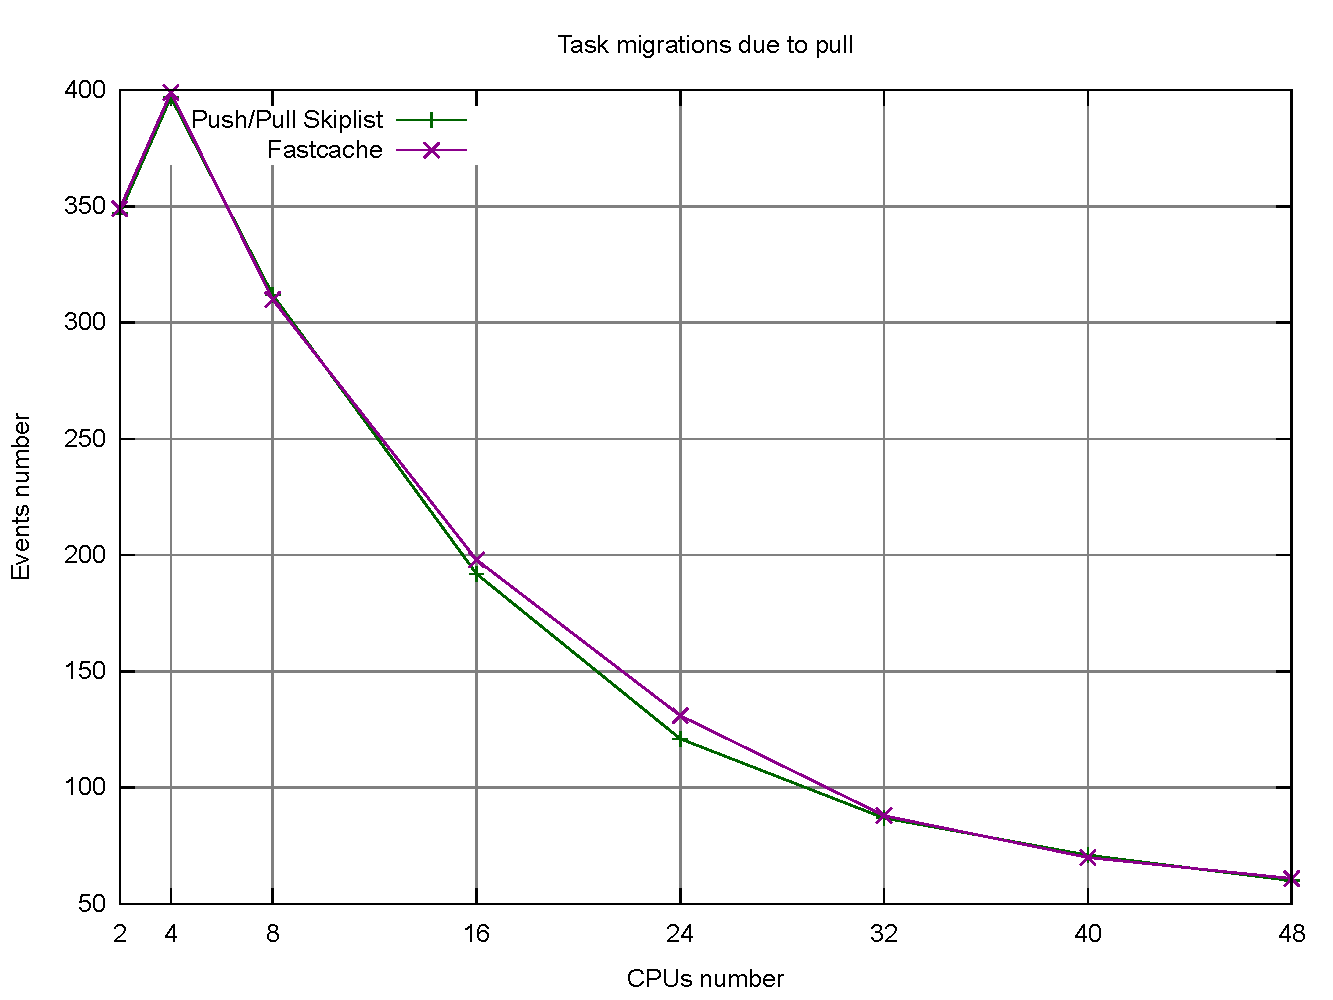
\includegraphics[width=\columnwidth]{images/fastcache_pulled_here}
    \caption{Number of task migrations due to pull operation}
    \label{fig:fastcache_pulled_here}
\end{figure}

Recall from Figures~\ref{fig:cpudl_push} and \ref{fig:cpudl_pull}
how the push and pull operations work: the former
has to cope with the \texttt{curr} deadline tasks, while the latter keeps
track of the \texttt{next} deadline tasks. This means that is easier, for
the pull \texttt{cpudl} data structure, to have an higher number of empty
items: that is, CPUs with no \texttt{next} deadline tasks. This condition
leads to an higher percentage of \emph{set} operations with the flag
\texttt{is\_valid} set to zero, thus an higher percentage of cache
invalidations. Since the slow path has to be followed more frequently for
the pull related \emph{set} operation, fastcache tends to be slightly dependent 
on the number of underlying CPUs. However, we can see that with an higher
number of CPUs fastcache performs better than the skip list. So we can state 
that fastcache scales better than the skip list.

Finally, from these latest figures, we can see that the number of task
migrations is about the same for max-heap, skip list and fastcache.
